\chapter{Testy eksperymentalne}
\label{chap:Testy eksperymentalne}

Chcąc przetestować praktyczne zastosowanie trójosiowego czujnika ruchu, oraz metod fuzji sygnałów na potrzeby sterowania robotem balansującym przeprowadzono, następujące testy:
\begin{itemize}
	\item test filtrów podczas jazdy
	\item wpływ silników na magnetometr
	\item stabilność odczytów
\end{itemize}

Wszystkie wymienione powyżej testy mają na celu sprawdzić, czy opisane w poprzednich rozdziałach metody przetwarzania danych z czujników ruchu oraz metody ich fuzji, wraz z zaimplementowanym algorytmem sterowania, są w stanie utrzymać opisaną w rozdziale \ref{chap:budowa} konstrukcję w okolicach punktu równowagi. Był to cel minimum, który musiała spełnić konstrukcja, aby można było uznać jej budowę za zakończoną sukcesem. 

Przyjęte parametry edytowane z poziomu aplikacji opisanej w rozdziale \ref{chap:aplikacja}, które doświadczalnie uznano za najbardziej optymalne są przedstawione w tabeli \ref{Parametry regulatorow PID} dotyczącej regulatorów PID, oraz w tabeli \ref{Parametry filtrow} dotyczącej filtrów.

\begin{table}[h!]
    \caption{Parametry regulatorów PID}
    \centering
    \begin{tabular}{|c|c|}
    \hline
    \multicolumn{2}{|c|}{Regulator prędkości} \\ \hline
    Kp                   & 20                  \\ \hline
    Ki                   & 60                  \\ \hline
    Kd                   & 0.1                  \\ \hline
    \hline
    \multicolumn{2}{|c|}{Regulator wychylenia} \\ \hline
    Kp                   & 100                   \\ \hline
    Ki                   & 10                   \\ \hline
    Kd                   & 0.1                   \\ \hline
    \end{tabular}
	\label{Parametry regulatorow PID}
\end{table}

\begin{table}[h!]
    \caption{Parametry filtrów}
    \centering
    \begin{tabular}{|c|c|}
    \hline
    \multicolumn{2}{|c|}{Filtr komplementarny} \\ \hline
    Parametr $\alpha$              & 0.001              \\ \hline
    \hline
    \multicolumn{2}{|c|}{Filtr Kalmana} \\ \hline
    Wariancja procesu & 1000           \\ \hline
    Wariancja pomiaru & 0.000001       \\ \hline
    \hline
    \multicolumn{2}{|c|}{Filtr Madgwicka} \\ \hline
    Parametr $\beta$              & 0.01              \\ \hline
    \end{tabular}
	\label{Parametry filtrow}
\end{table}

%----------------------------------------------------------------------------------------------------------------
\section{Wpływ silników na magnetometr}

Pierwszy przeprowadzony test miał na celu sprawdzenie poprawności wyznaczanych kątów RPY podczas jazdy. Poprawność wyznaczonych kątów określana była doświadczalnie na podstawie wykresów w aplikacji.

Efekt przeprowadzonego testu, którego wynik jest negatywny przedstawiono na wykresie \ref{Silniki magnetometr}. Na wykresie oznaczono dwa momenty podczas wykonywania testu. Pierwszy z nich to moment załączenia silników z maksymalną prędkością na poziomie 180 RPM. Po włączeniu, widoczne są okresowe zmiany wyznaczonego na podstawie odczytów z magnetometru kąta Yaw. Są one związane ze zmiennym polem magnetycznym, generowanym przez zwoje silników krokowych. Drugi moment oznaczony na wykresie, to wyłączenie napędu, po którym zakłócenia znikają. 

\begin{figure}[h!]
    \centering
    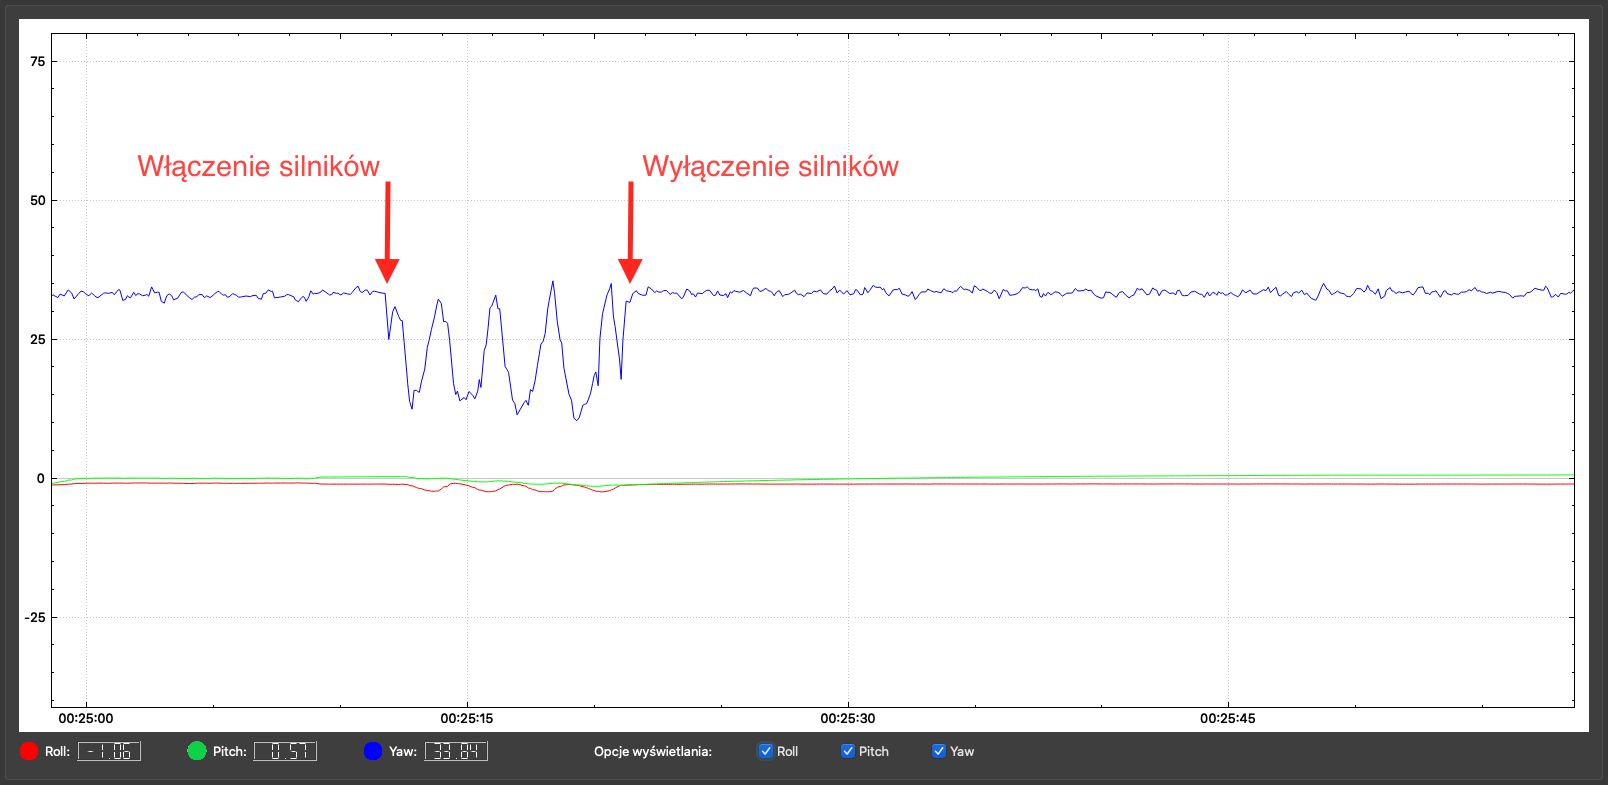
\includegraphics[width=1\textwidth]{Rysunki/Rozdzial07/Wplyw_silnikow_magnetometr.png}
    \caption{Wykres przedstawiający zakłócenia wywołane pole magnetycznym wytwarzanym przez silniki}
    \label{Silniki magnetometr}
\end{figure}

Całość spowodowana był zbyt małą odległością pomiędzy czujnikiem, a silnikami, która wynosiła około 12 cm. Gdyby, wyznaczony w taki sposób kąt Yaw brał udział w algorytmie sterowania, uniemożliwiłby on jego poprawne działanie. Chcąc wyeliminować ten błąd, należałoby zwiększyć odległość między czujnikiem a silnikami, lub skorzystać z samego żyroskopu.
%----------------------------------------------------------------------------------------------------------------
\section{Stabilność odczytów}

Kolejny z przeprowadzonych testów, miał na celu sprawdzenie czy kąty RPY dla trzech zaimplementowanych filtrów nie zaczynają różnić się znacząco między poszczególnymi odstępami czasu. Są to wartości czasu mierzone od początku działania programu sterującego robotem.

Pierwszy test został przeprowadzony z wyłączonymi silnikami oraz z unieruchomionym robotem. Wyniki testu przedstawione są w tabeli \ref{Tabela brak ruchu}, z której wynika, że nie zaobserwowano znaczącej różnicy dla wartości kątów wyznaczonych w pierwszej oraz piętnastej minucie trwania testu.

\begin{table}[h!]
    \centering
    \caption{Odczyty dla poszczególnych filtrów przy braku ruchu}
    \begin{tabular}{|c|c|c|c|}
        \hline
        Czas [min.] & F.Komplementarny [R/P/Y] & F.Kalmana [R/P/Y] & F.Madgwicka [R/P/Y] \\
        \hline
        1 & -1.25 / -0.79 / 30.67 & -1.26 / -1.32 / 31.48 & -1.26 / -0.28 / 29.87 \\
        \hline
        2 & -1.26 / -1.09 / 30.96 & -1.24 / -0.14 / 30.83 & -1.28 / -0.25 / 29.17  \\
        \hline
        5 & -1.27 / -0.96 / 30.15 & -1.22 / -0.15 / 30.77 & -1.23 / -0.28 / 29.38  \\
        \hline
        10 & -1.26 / -0.95 / 30.27 & -1.28 / -0.12 / 30.75 & -1.26 / -0.26 / 29.78  \\
        \hline
    \end{tabular}
	\label{Tabela brak ruchu}
\end{table}

Drugi test, został przeprowadzony dla robota swobodnie balansującego, bez zadanej prędkości silników. Wyniki przeprowadzonego testu zaprezentowano w tabeli \ref{Tabela ruch}. W tym przypadku również nie zaobserwowano znaczących różnic w wyznaczanych wartościach w pierwszej i piętnastej minucie testu, oprócz kąta Yaw, którego odczyty nie są do końca poprawne ze względu na wypływ działających silników.

\begin{table}[h!]
    \centering
    \caption{Odczyty dla poszczególnych filtrów podczas balansowania w miejscu}
    \begin{tabular}{|c|c|c|c|}
        \hline
        Czas [min.] & F.Komplementarny [R/P/Y] & F.Kalmana [R/P/Y] & F.Madgwicka [R/P/Y] \\
        \hline
        1 & -1.27 / -1.48 / 30.74 & -1.46 / -0.37 / 23.82 & -0.79 / 0.66 / 25.18 \\
        \hline
        2 & -1.33 / -1.62 / 28.43 & -1.51 / -0.22 / 23.22 & -0.75 / 0.64 / 24.92  \\
        \hline
        5 & -1.24 / -1.44 / 28.92 & -1.55 / -0.44 / 23.51 & -0.76 / 0.47 / 23.24  \\
        \hline
        10 & -1.16 / -1.1 / 27.79 & -1.56 / -0.23 / 25.06 & -0.85 / 1.19 / 24.87  \\
        \hline
    \end{tabular}
	\label{Tabela ruch}
\end{table}

Pozytywny wynik przeprowadzonego testu potwierdza możliwość zastosowania tej implementacji na rzeczywistym robocie. Nie powinny mieć miejsca żadne dryfowania odczytów, co uniemożliwiałoby utrzymywanie robota w okolicach punktu równowagi oraz powodowałyby dryf pozycji robota.

%----------------------------------------------------------------------------------------------------------------
\section{Test filtrów podczas jazdy}

Po przetestowaniu poprawności odczytów kątów RPY, postanowiono sprawdzić jak robot radzi sobie z jazdą. W algorytmie sterowania bierze udział, tylko kąt Pitch, dlatego postanowiono wyłączyć wyświetlanie na wykresie pozostałych kątów. Test dla każdego filtru wykonany został osobno, ze względu na brak możliwości uruchomienia trzech algorytmów jednocześnie, w połączeniu z algorytmem sterowania (zbyt mała moc obliczeniowa mikrokontrolera). 

\subsection{Zwykła jazda}

Test polegał, na sprawdzeniu czy robot jest w stanie balansować, czy jest odporny na zewnętrzne zakłócenia, np. w postaci pchnięcia ręką, oraz radzenie sobie z zadawaną prędkością obrotową kół (jazda w przód i w tył). Moment pchnięcia oraz wykonania jazdy w przód i w tył oznaczone zostały na wykresach \ref{Wykresy filtry test}.

Wynik przeprowadzonego jest pozytywny, ponieważ pozycja robota stabilizuje się, zarówno po pchnięciu robota jak i po zakończeniu jazdy w przód i w tył dla wszystkich trzech algorytmów. Czasy stabilizacji nieznacznie się różnią od siebie, dla tak dobranych parametrów regulatorów oraz filtrów.
 
\begin{figure}[h!]
    \centering
    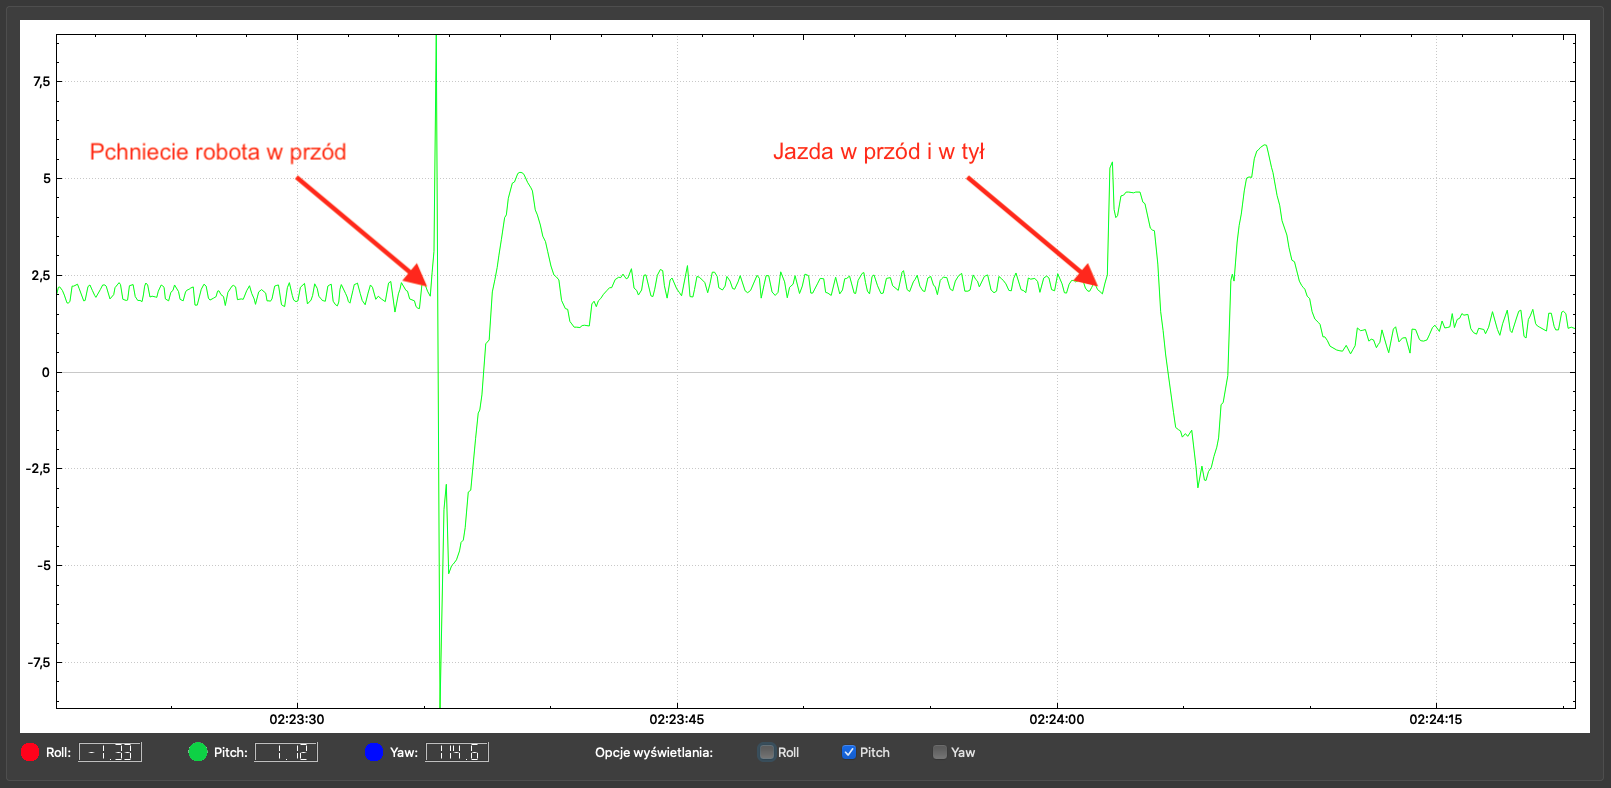
\includegraphics[width=1\textwidth]{Rysunki/Rozdzial07/Komplementarny_jazda.png}
    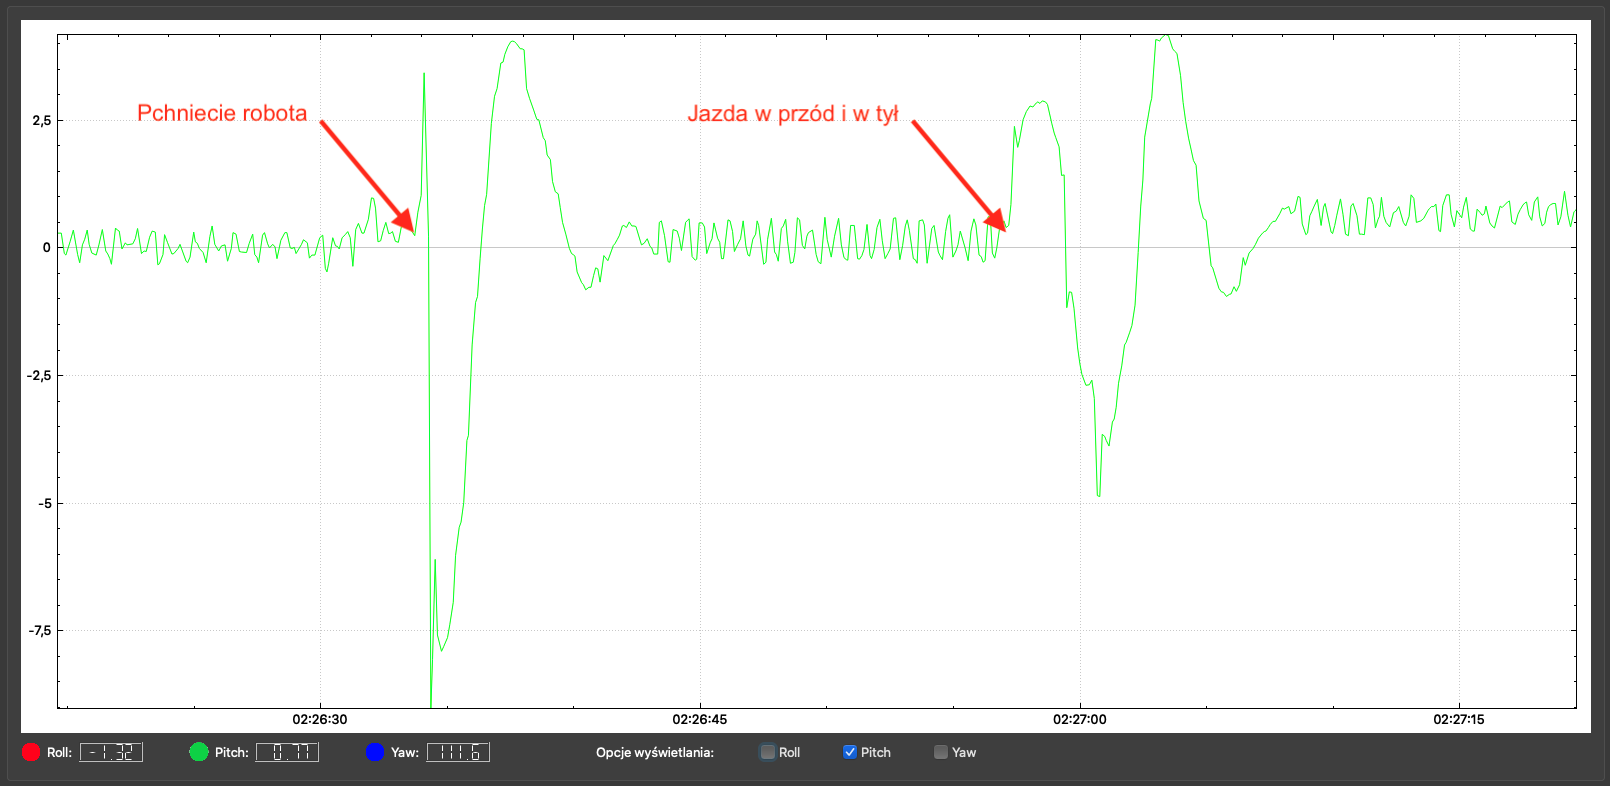
\includegraphics[width=1\textwidth]{Rysunki/Rozdzial07/Kalman_jazda.png}
    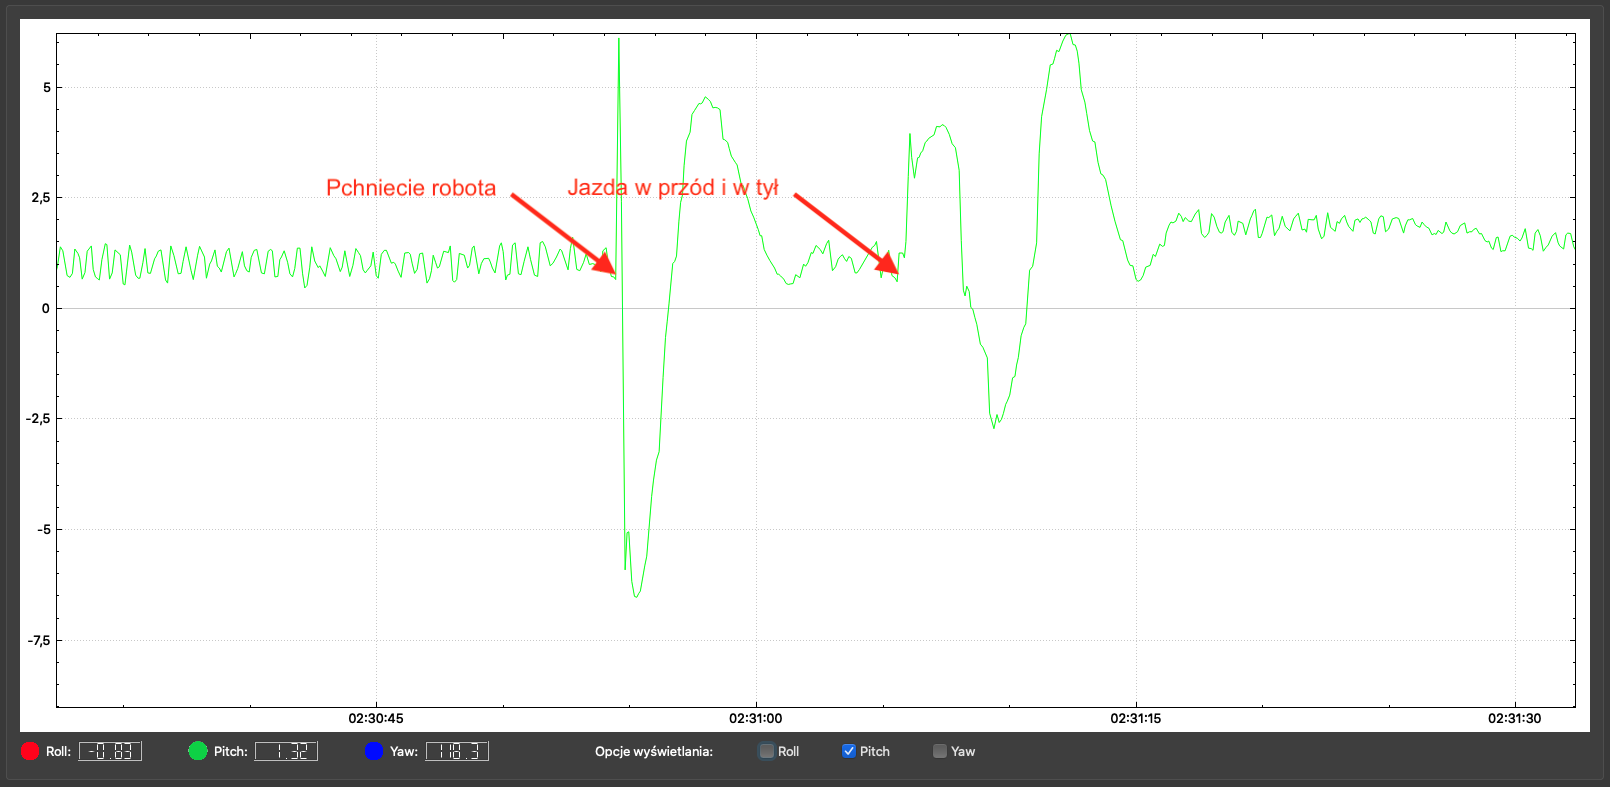
\includegraphics[width=1\textwidth]{Rysunki/Rozdzial07/Madgwick_jazda.png}
    \caption{Wykresy kąta Pitch dla filtrów, od góry: Komplementarnego, Kalmana, Madgwicka}
    \label{Wykresy filtry test}
\end{figure}

\subsection{Balansowanie z ładunkiem}

Zechciano sprawdzić jeszcze jak robot radzi sobie z balansowaniem, po dołożeniu obciążenia, w tym wypadku w postaci plastikowej butelki z wodą o pojemności 1.5 litra. Wyniki testu przedstawiono na wykresach \ref{Z butelka wykresy}, wraz z załączoną fotografią \ref{Z butelka} wykonaną podczas przeprowadzania testu. Wynik testu, jest pozytywny pod względem tego, że robot nie utracił równowagi i nie wywrócił się. Pojawiły się natomiast oscylacje związane z oddaleniem środka masy od osi obrotu takiego układu od układu bez obciążenia. Chcąc wyeliminować oscylacje należałoby zaimplementować regulator reagujący na zmienne parametry modelu, np. z wykorzystaniem algorytmu Fuzzy Logic.

\begin{figure}[h!]
    \centering
    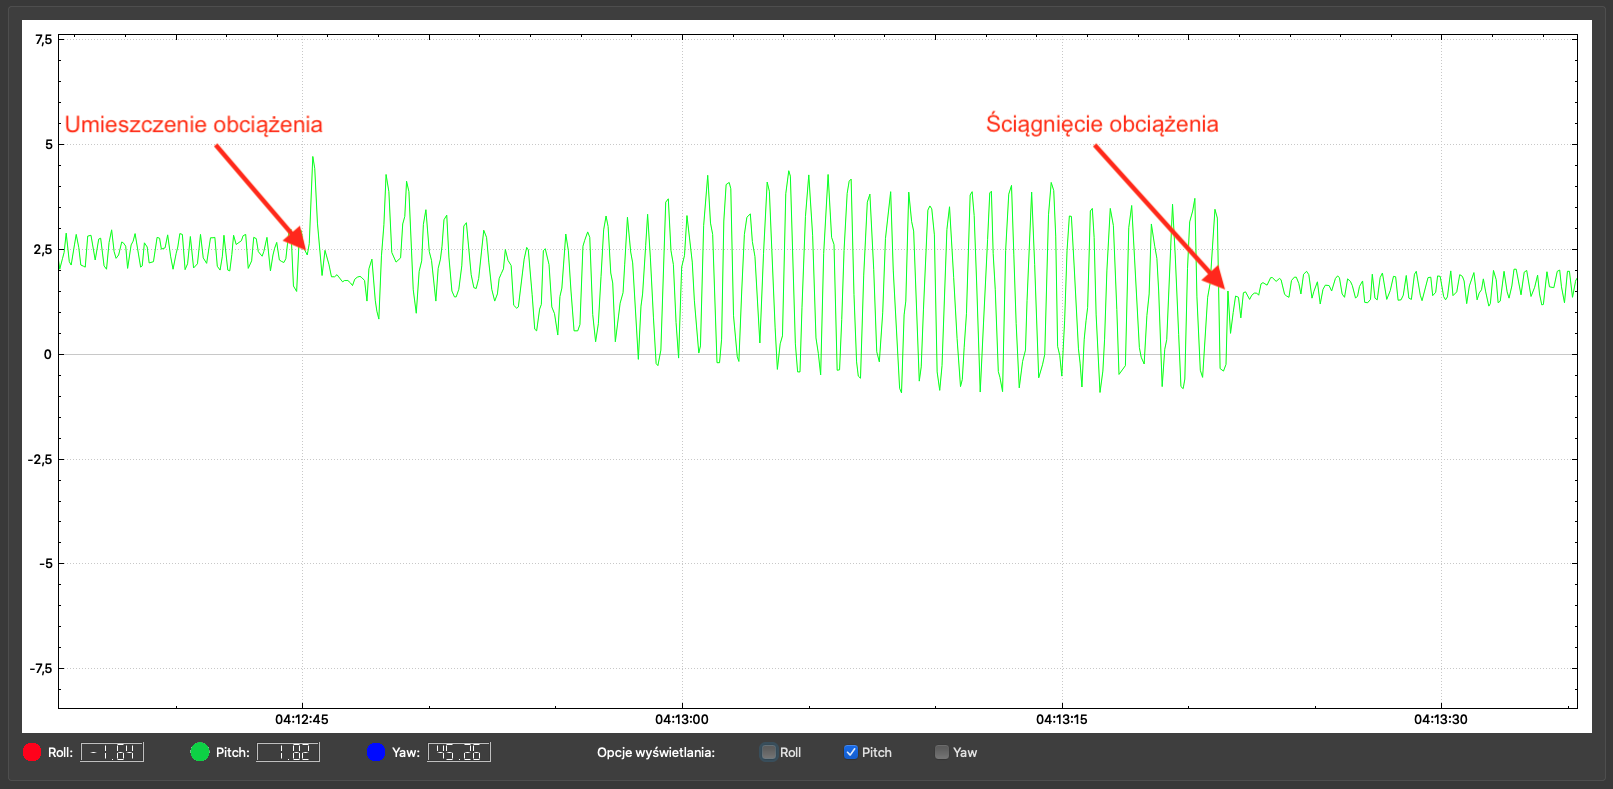
\includegraphics[width=1\textwidth]{Rysunki/Rozdzial07/Komplementarny_butelka.png}
    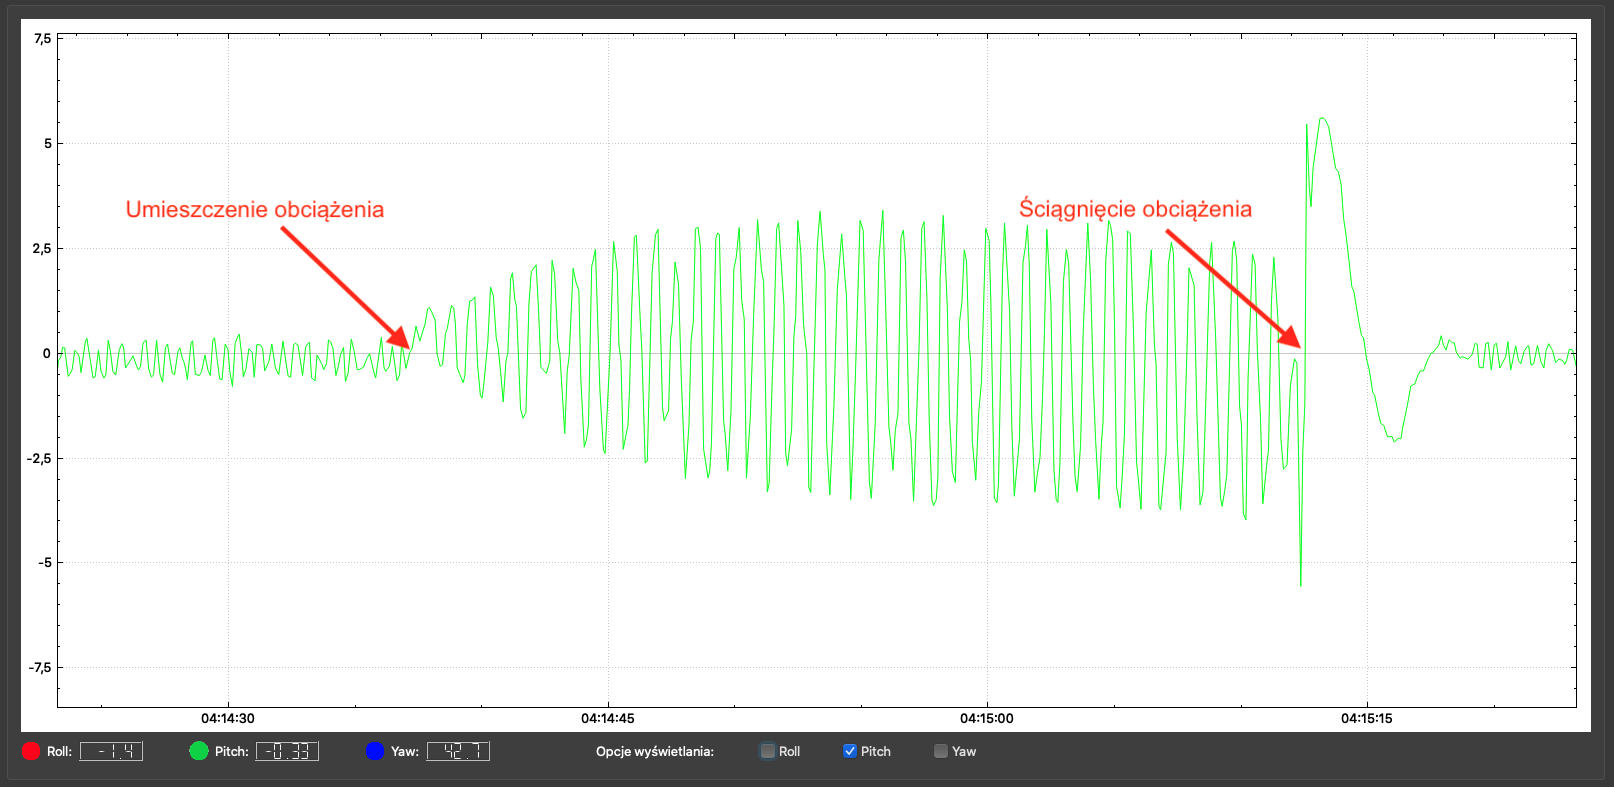
\includegraphics[width=1\textwidth]{Rysunki/Rozdzial07/Kalman_butelka.png}
    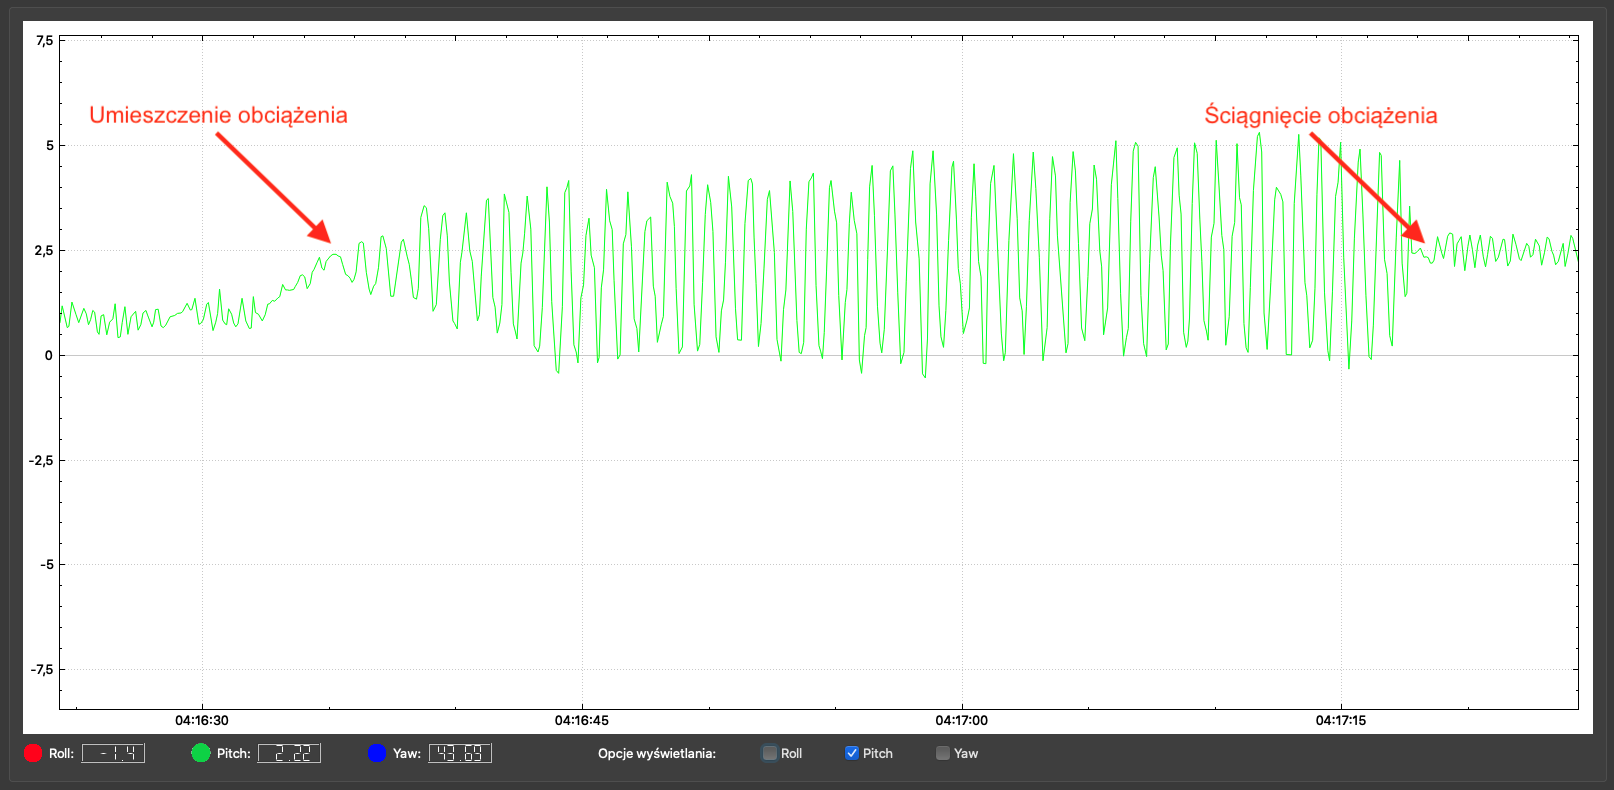
\includegraphics[width=1\textwidth]{Rysunki/Rozdzial07/Madgwick_butelka.png}
    \caption{Wykresy kąta Pitch dla filtrów, od góry: Komplementarnego, Kalmana, Madgwicka z butelką umieszczoną na górze robota}
    \label{Z butelka wykresy}
\end{figure}

\begin{figure}[h!]
    \centering
    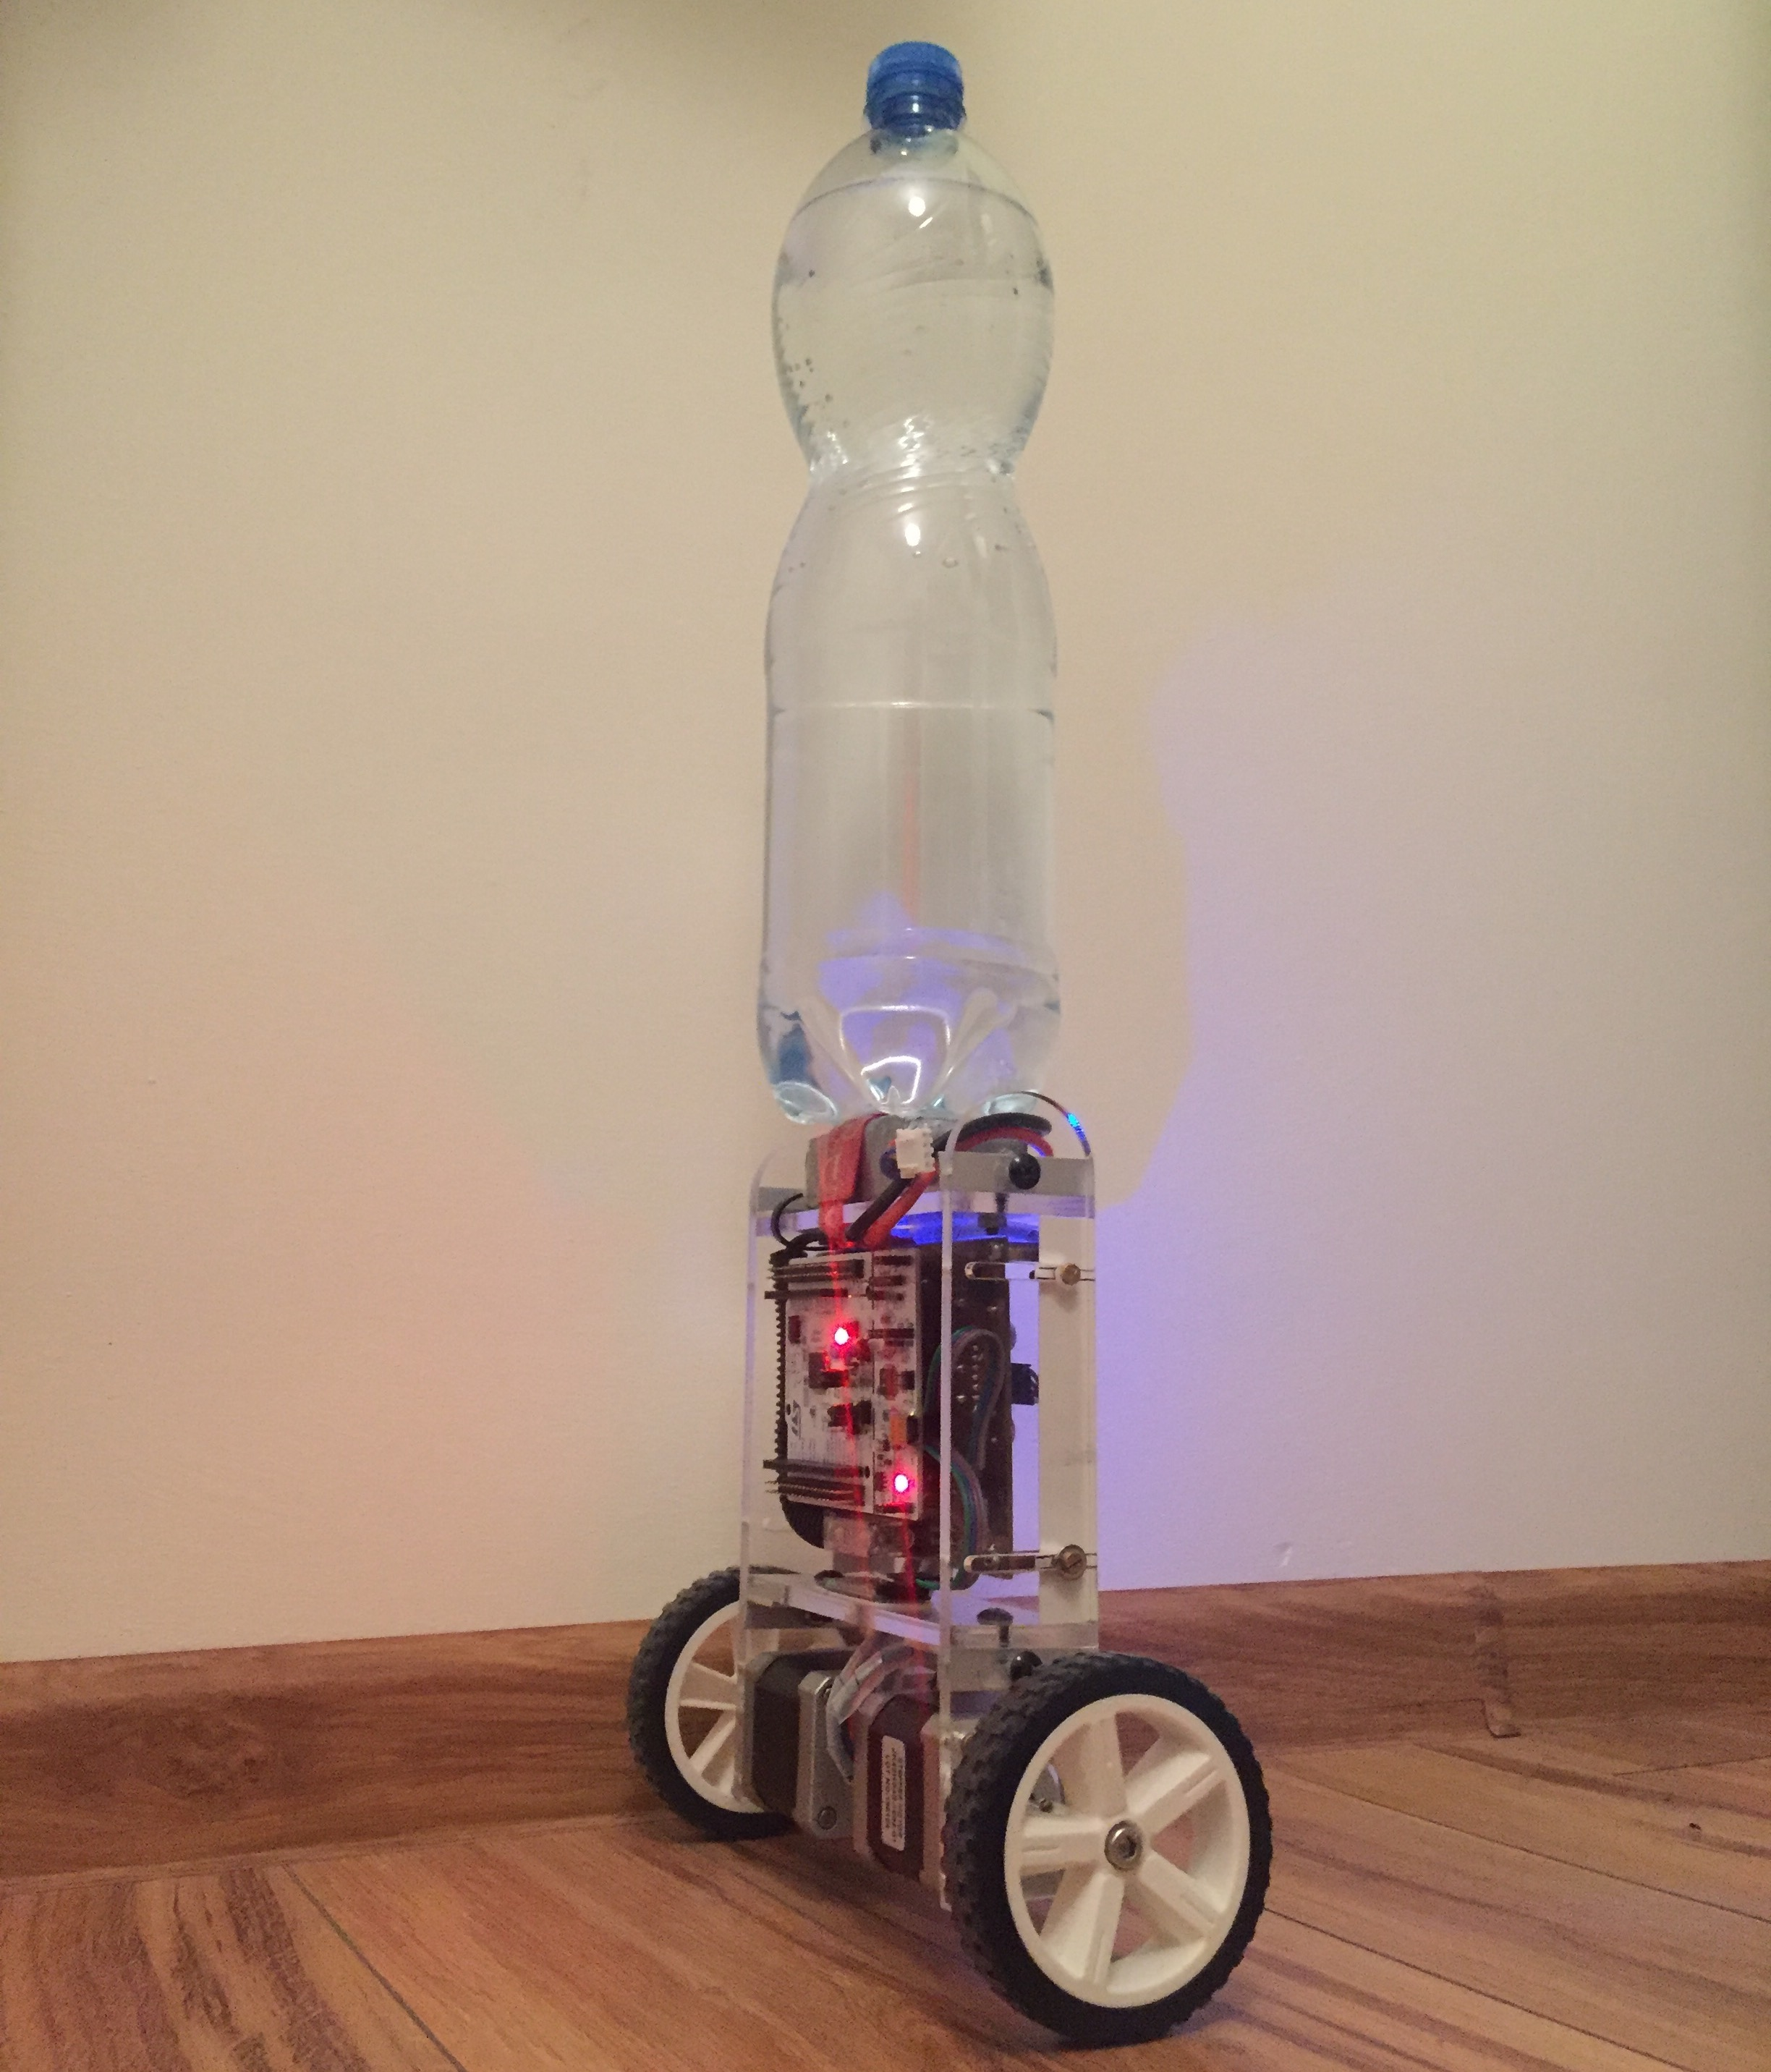
\includegraphics[width=1\textwidth]{Rysunki/Rozdzial07/Butelka_zdjecie.png}
    \caption{Fotografia robota podczas balansowania z obciążeniem w postaci butelki z wodą}
    \label{Z butelka}
\end{figure}

%----------------------------------------------------------------------------------------------------------------
\section{Test czujników w systemie OptiTrack}

\texttt{OptiTrack}(Motion Capture) jest systemem wykorzystywanym do rejestrowania ruchu obiektów, do których zamocowano specjalne markery. Są one wykonane z wysokopołyskliwej folii, która odbija promieniowanie podczerwone generowane przez diody umieszczone na kamerach. Na podstawie odbitego promieniowania podczerwonego, które trafia do oka kamery wyznaczana jest aktualna pozycja markera oraz pozycja i orientacja markerów połączonych w jeden obiekt. Najczęstszym zastosowaniem tego systemu, jest tworzenie animacji komputerowej w grach bądź filmach, na podstawie ruchów aktorów wyposażonych w kostiumy z rozmieszczonymi na swej powierzchni markerami.

Technologię tę postanowiono wykorzystać do sprawdzenia poprawności kątów estymowanych przez trzy opisane w tej pracy algorytmy. Rysunek \ref{Wykresy OptiTrack RPY} przedstawia trzy wykresy z zarejestrowanymi danymi z mikrokontrolera obsługującego czujniki ruchu, a także z oprogramowania \texttt{Motive}. Dane dotyczyły rotacji w trzech osiach metalowego stelażu, na którym dodatkowo umieszczono markery, a także czujniki ruchu wraz mikrokontrolerem oraz modułem \texttt{Bluetooth} przesyłającym dane do komputera. 

Kolory danych na wykresach:
\begin{itemize}
    \item czerwony -- filtr komplementarny
    \item zielony -- filtr Kalmana
    \item niebieski -- filtr Madgwicka
    \item fioletowy -- system OptiTrack
\end{itemize}

\begin{figure}[h!]
    \centering
    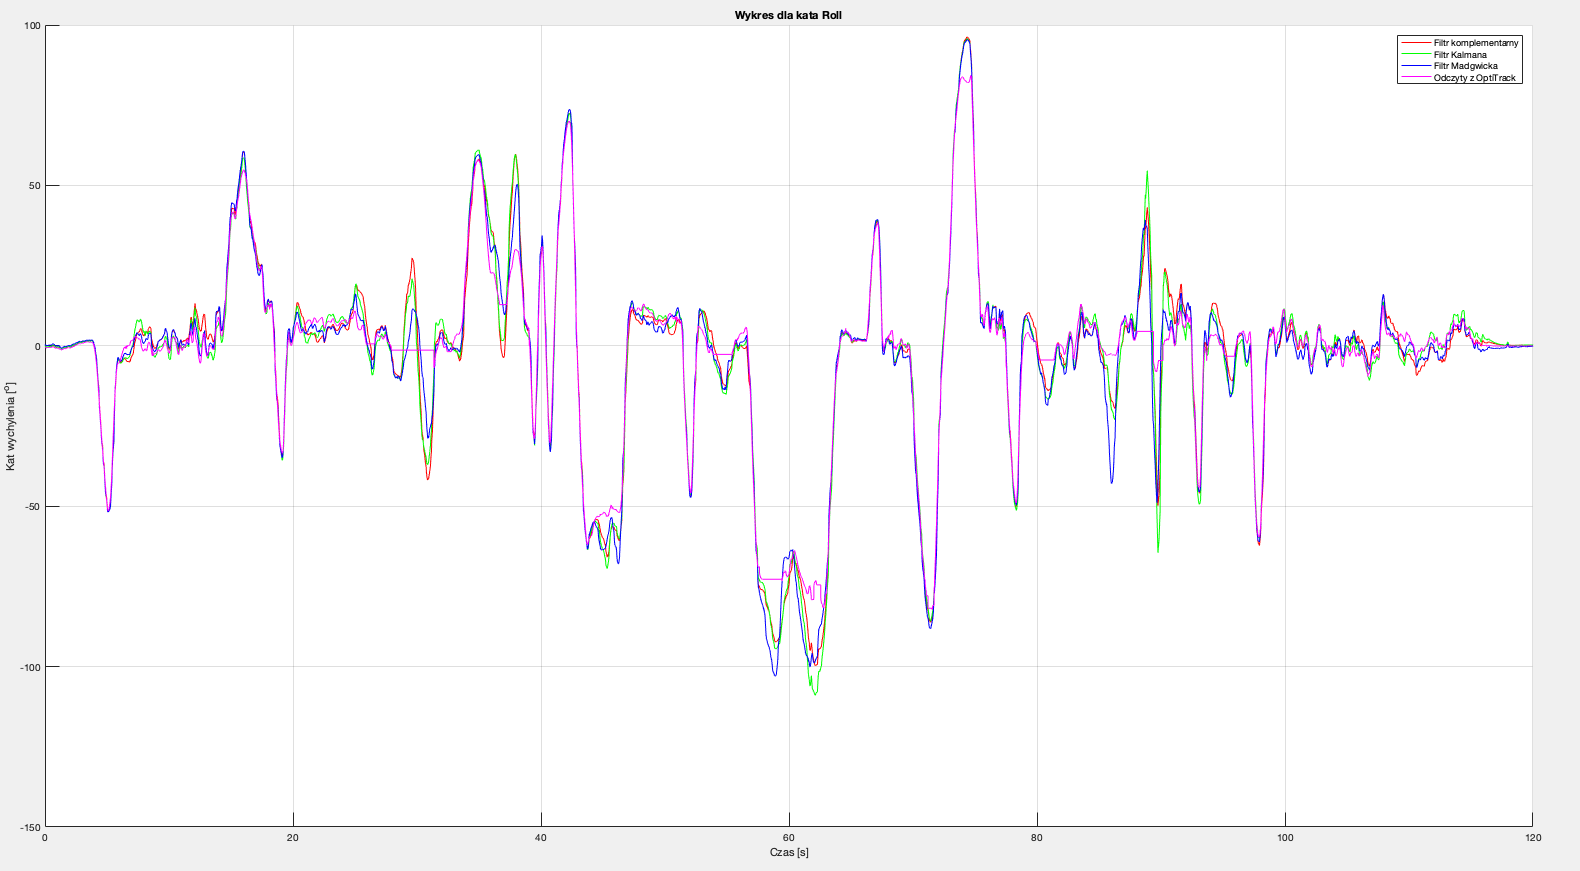
\includegraphics[width=0.9\textwidth]{Rysunki/Rozdzial07/OptiTrack_Roll_wykres.png}
    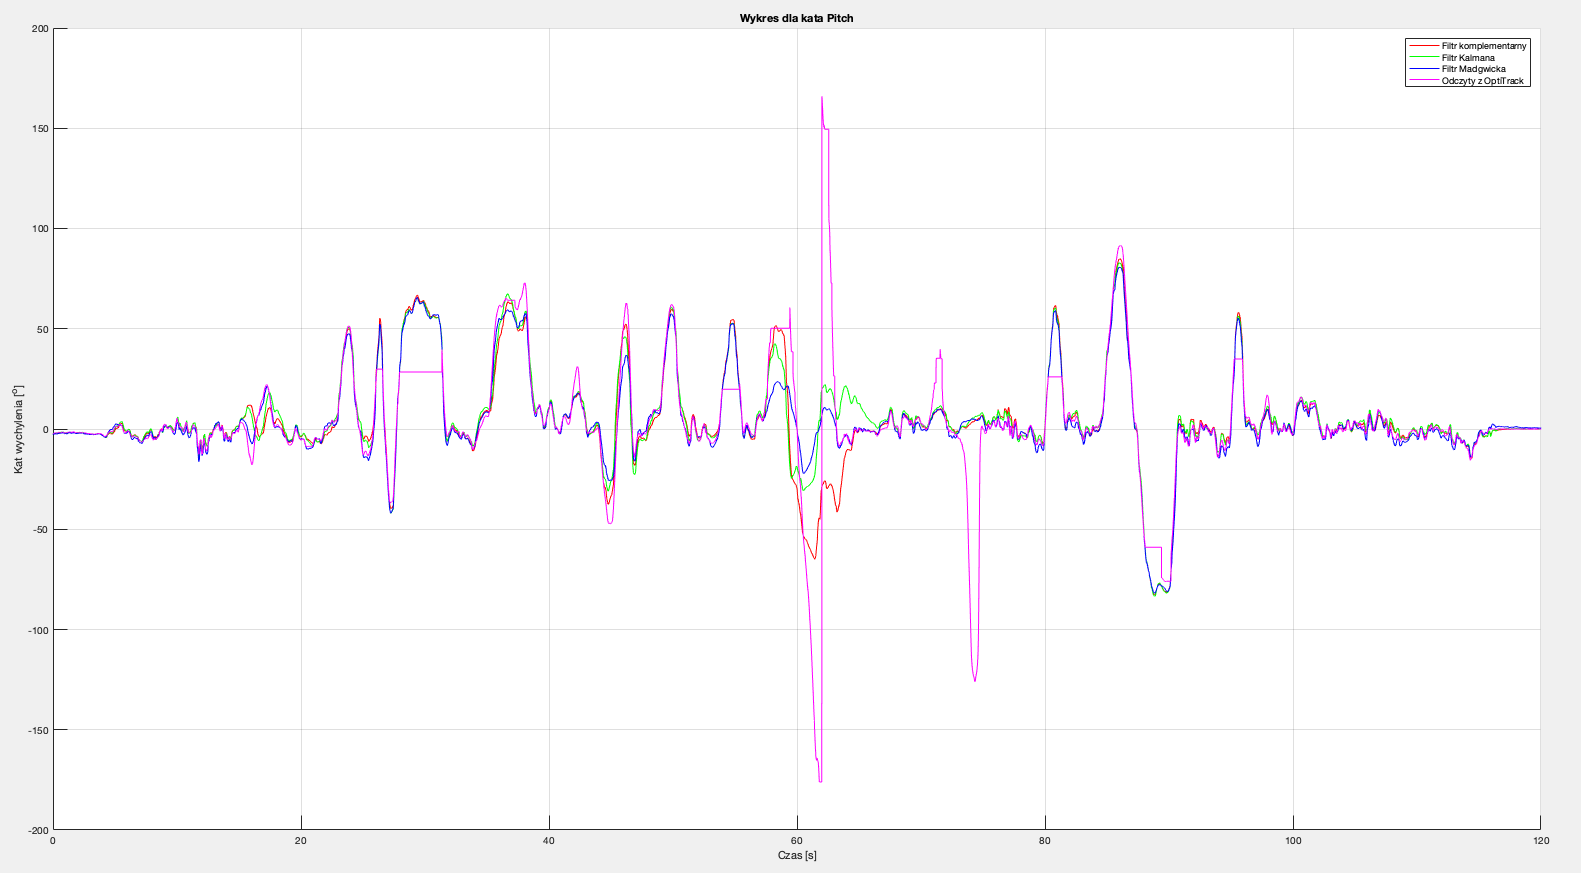
\includegraphics[width=0.9\textwidth]{Rysunki/Rozdzial07/OptiTrack_Pitch_wykres.png}
    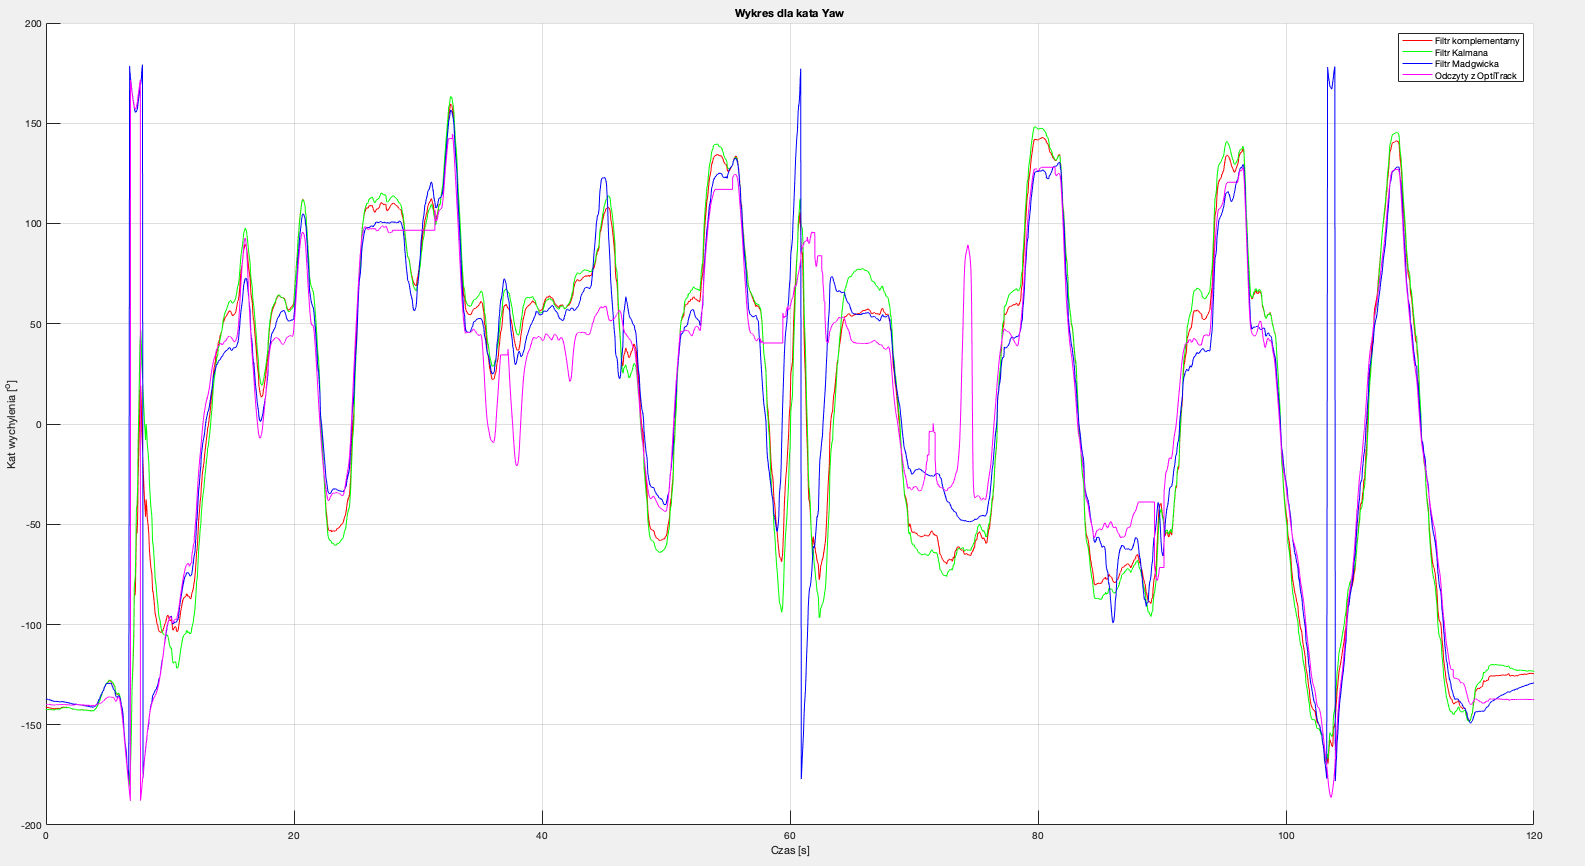
\includegraphics[width=0.9\textwidth]{Rysunki/Rozdzial07/OptiTrack_Yaw_wykres.png}
    \caption{Wykresy dla przeprowadzonego testu w systemie OptiTrack: Roll, Pitch, Yaw}
    \label{Wykresy OptiTrack RPY}
\end{figure}

Przeprowadzony test zakończył się powodzeniem, ponieważ udało się zsynchronizować i porównać dane zarejestrowane przez dwa niezależne systemy. W danych zarejestrowanych przez system \texttt{OptiTrack}, w niektórych miejscach na wykresie pojawiają się zakłócenia w postaci nagłych skoków wartości lub odczyt niezmieniający się w czasie przez około 5 sekund. Prawdopodobną przyczyną występowania zakłóceń był brak idealnych warunków oświetleniowych podczas testowania (nadmiernie oświetlone pomieszczenie) oraz nie przewidziano sytuacji, w której jeden z markerów znika z pola widzenia kamer w wyniku zasłonięcia przez metalowy stelaż lub fragment ciała osoby przeprowadzającej test. Wartości estymowanych kątów można byłoby polepszyć poprzez zmianę parametrów poszczególnych filtrów, zwiększenie czasu próbkowania i dokładności obliczeń oraz zastosowanie wysokiej jakości oryginalnych czujników. 

%----------------------------------------------------------------------------------------------------------------
\section{Podsumowanie}

Celem zrealizowanego projektu było porównanie przydatności wybranych metod fuzji sygnałów na potrzeby sterowania robotem balansującym. Wszystkie trzy metody z powodzeniem zostały zaimplementowane i przetestowane. Najpierw symulacyjnie w środowisku \texttt{Matlab}, następnie na rzeczywistym robocie w pętli sprzężenia zwrotnego sterowania, a na koniec w ramach dodatkowego eksperymentu z zastosowaniem technologii \texttt{Motion Capture} pełniącego rolę systemu referencyjnego. Podczas sterowania robotem, nie zauważono znaczących różnic pomiędzy wykorzystaniem w algorytmie sterowania filtru komplementarnego, Kalmana czy Madgwicka. Ponadto analiza modelu dynamiki robota i przeprowadzone symulacje w znacznym stopniu ułatwiły etap implementacji i strojenia algorytmu sterowania.

W ramach udoskonalenia projektu, można byłoby zmienić algorytm sterowania implementując sterownik adaptacyjny, tak aby poprawić jakość regulacji niwelując oscylacje, które pojawiają się w momencie dołożenia dodatkowego obciążenia na robocie. Sterownik adaptacyjny dobierałby swoje parametry w zależności od parametrów modelu, głównie momentu bezwładności wahadła. Kolejną rzeczą jaką należałoby udoskonalić jest zbyt duży wpływ pola magnetycznego na odczyty pochodzące z magnetometru. Jednym z rozwiązań mogłoby być wydłużenie samego wahadła, a co za tym idzie oddalenie czujnika od silników. 

Wszystkie cele i założenia projektowe zostały z powodzeniem zrealizowane, a rezultaty przeprowadzonych testów są zadowalające z wyjątkiem negatywnego wpływu silników w trakcie pracy na magnetometr, którego niestety nie udało się wyeliminować gdyż wymagałoby to przebudowy całej konstrukcji.

%----------------------------------------------------------------------------------------------------------------